% !TEX root = saveliev_physics_general_course_1.tex
%!TEX TS-program = pdflatex
%!TEX encoding = UTF-8 Unicode

\appendix

\chapter*{APPENDICES}\label{chap:A}
\addcontentsline{toc}{chapter}{APPENDICES}
\chaptermark{APPENDICES}
\renewcommand{\thechapter}{A}
\setcounter{section}{0}
\renewcommand{\thesection}{\thechapter.\arabic{section}}
% \setcounter{theorem}{0}
% \renewcommand{\thetheorem}{\thechapter.\arabic{theorem}}
\setcounter{equation}{0}
\renewcommand{\theequation}{\thechapter.\arabic{equation}}
\setcounter{figure}{0}
% \setcounter{table}{0}

\section{List of Symbols}\label{sec:A_1}

\begin{table}[h]
	% \renewcommand{\arraystretch}{1.2}
	% \caption{ }
	% \vspace{-0.6cm}
	% \label{table:12_1}
	\begin{center}\resizebox{\linewidth}{!}{
        \begin{threeparttable}[b]
			\begin{tabular}{p{0.5cm} p{11cm}}
                $A$ & amplitude; atomic mass; work\\
                $a$ &  distance\\
                $\vec{a}$ & acceleration\tnote{${\dagger}$}$\,\,$; vector\\
                $B$ & amplitude\\
                $b$ & distance; thickness\\
                $\vec{b}$ & vector\\
                $C$ &  curvature; molar heat capacity\\
                $c$ &  distance; relative concentration; specific heat capacity; speed of light\\
                $\vec{c}$ &  vector\\
                $D$ &  diffusion coefficient\\
                $d$ &  collision diameter; diameter\\
                $\vec{d}$ &  vector\\
                $E$ &  energy; mechanical equivalent of heat; Young's modulus\\
                $e$ &  base of natural logarithms\\
                $\hatvec{e}$ &  unit vector\\
                $F$ &  free (Helmholtz) energy\\
                $\vec{F}$ &  force\\
                $\vec{F}^*$ & non-conservative force\\
                $f$ &  coefficient of friction; relative fluctuation\\
                $\vec{f}$ &  force\\
                % $G$ &  Gibbs thermodynamic potential (Gibbs energy); gravitational constant; shear modulus\\
                % $\vec{g}$ &  acceleration of free fall\\
                % $\vec{g}'$ &  gravitational field vector, gravitational intensity\\
               % $H$ &  curvature; enthalpy\\
               % $h$ &  height; Planck's constant\\
               % $\hbar$ &  Planck's constant divided by $2\pi$ ($h/2\pi$)\\
               % $I$ &  moment of inertia\\
               % $\Im$ & imaginary\\
               % $i$ & imaginary unity ($i=\sqrt{-1}$)\\
               % $K$ & momentum (also $p$); momentum flux\\
               % $k$ & Boltzmann constant; constant of proportionality; quasi-elastic force coefficient; spring constant\\
               % $L$ & heat of transition
			\end{tabular}
            \begin{tablenotes}
    			\item [${\dagger}$] The magnitude of a vector is denoted by the same symbol as the vector itself, but in ordinary italic (sloping) type.
    		\end{tablenotes}
        \end{threeparttable}
	}\end{center}
\end{table}

\begin{table}[h]
	% \renewcommand{\arraystretch}{1.2}
	% \caption{ }
	% \vspace{-0.6cm}
	% \label{table:12_1}
	\begin{center}\resizebox{\linewidth}{!}{
			\begin{tabular}{p{0.5cm} p{11cm}}
                $G$ &  Gibbs thermodynamic potential (Gibbs energy); gravitational constant; shear modulus\\
                $\vec{g}$ &  acceleration of free fall\\
                $\vec{g}'$ &  gravitational field vector, gravitational intensity\\
                $H$ &  curvature; enthalpy\\
                $h$ &  height; Planck's constant\\
                $\hbar$ &  Planck's constant divided by $2\pi$ ($h/2\pi$)\\
                $I$ &  moment of inertia\\
                $\Im$ & imaginary\\
                $i$ & imaginary unity ($i=\sqrt{-1}$)\\
                $K$ & momentum (also $p$); momentum flux\\
                $k$ & Boltzmann constant; constant of proportionality; quasi-elastic force coefficient; spring constant\\
                $L$ & heat of transition\\
                $\vec{L}$ & angular momentum\\
                L & dimension of length\\
                $l$ & length; mean free path of molecule\\
                $M$ & mass\\
                $\vec{M}$ & moment of force (torque)\\
                M & dimension of mass\\
                $m$ & mass\\
                $N$ & number of molecules, particles, etc.\\
                $\ab{N}{A}$ & Avogadro constant\\
                $n$ & number of molecules or particles per unit volume; polytropic exponent\\
                $p$ & power; probability\\
                $\vec{P}$ & force of gravity\\
                $p$ & pressure\\
                $\vec{p}$ & momentum (also $\vec{K}$)\\
                $Q$ & amount of heat; quality; rate of flow\\
                $q$ & heat flux\\
                $R$ & molar gas constant; radius of curvature\\
                $\reynolds$ & Reynolds number\\
                $\Re$ & real\\
                $r$ & radius; resistance coefficient\\
                $\vec{r}$ & displacement; position (radius) vector\\
                $S$ & area; entropy\\
                $s$ & distance; "interval"\\
			\end{tabular}
	}\end{center}
\end{table}

\begin{table}[h]
	% \renewcommand{\arraystretch}{1.2}
	% \caption{ }
	% \vspace{-0.6cm}
	% \label{table:12_1}
	\begin{center}\resizebox{\linewidth}{!}{
			\begin{tabular}{p{0.5cm} p{11cm}}
                $T$ & absolute temperature; period of revolution\\
                T & dimension of time\\
                $t$ & temperature, Celsius scale; time\\
                $U$ & internal energy\\
                $u$ & velocity\\
                $V$ & potential function; volume\\
                $\vec{v}$ & velocity\\
                $\vec{W}$ & weight\\
                $w$ & energy density\\
                $x$ & coordinate\\
                $y$ & coordinate\\
                $z$ & complex number; coordinate\\
                $\alpha$ & angle; coefficient of elastic compliance; constant; initial phase of oscillations\\
                $\vec{\alpha}$ & angular acceleration\\
                $\beta$ & angle; damping factor; refrigerating factor (coefficient of performance)\\
                $\gamma$ & angle; ratio of heat capacities $C_p/C_V$; relative shear\\
                $\Delta$ & increment\\
                $\Delta'$ & elementary amount\\
                $\varepsilon$ & energy; strain\\
                $\eta$ & efficiency; viscosity (dynamic)\\
                $\Theta$ & thermodynamic temperature\\
                $\theta$ & angle; temperature\\
                $\varkappa$ & thermal conductivity coefficient\\
                $\Lambda$ & volume of cell in $v$-space\\
                $\lambda$ & logarithmic decrement\\
                $\mu$ & reduced mass\\
                $\nu$ & frequency; kinematic viscosity; number of revolutions per unit time\\
                $\pi$ & ratio of circumference to diameter, $\pi=3.14+$\\
                $\rho$ & density; polar coordinate\\
                $\sigma$ & effective section of molecule; stress; surface tension\\
                $\tau$ & proper time; tangential or shear stress\\
                $\hatvec{\tau}$ & unit vector of tangent to trajectory\\
                $\varphi$ & angle; polar coordinate\\
                $\Omega$ & solid angle; statistical weight\\
                $\omega$ & cyclic frequency\\
                $\vec{\omega}$ & angular velocity\\
			\end{tabular}
	}\end{center}
\end{table}

\clearpage


\section{Calculation of Selected Integrals}\label{sec:A_2}

$\quad$1. The improper integral
\begin{equation}\label{eq:A_1}
    I(\beta) = \int_{-\infty}^{+\infty} \exp\parenthesis{-\beta x^2}\,\deriv{x}
\end{equation}

\noindent
is called the \textit{Poisson integral}. Denoting the integration variable by the letter $y$, we can write this integral in the form
\begin{equation*}
    I(\beta) = \int_{-\infty}^{+\infty} \exp\parenthesis{-\beta y^2}\,\deriv{y}.
\end{equation*}

\noindent
Multiplying the two expressions, we arrive at the double integral
\begin{align}
    \bracket{I(\beta)}^2 &= \int_{-\infty}^{+\infty} \exp\parenthesis{-\beta x^2}\,\deriv{x} \int_{-\infty}^{+\infty} \exp\parenthesis{-\beta y^2}\,\deriv{y}\nonumber\\
    &= \int_{-\infty}^{+\infty}\int_{-\infty}^{+\infty} \exp\bracket{-\beta\parenthesis{x^2+y^2}}\,\deriv{x}\,\deriv{y}.\label{eq:A_2}
\end{align}

It is easy to calculate this integral by considering the variables $x$ and $y$ as Cartesian coordinates in a plane and passing over from these coordinates to the polar ones $r$ and $\varphi$. When $x$ and $y$ vary from $-\infty$ to $+\infty$, the coordinate $r$ varies within the limits from $0$ to $\infty$, and $\varphi$ within the limits from $0$ to $2\pi$.
The sum $x^2+y^2$ equals $r^2$, while the surface element $\deriv{x}\,\deriv{y}$ in polar coordinates has the form $r\,\deriv{r}\,\deriv{\varphi}$. Performing this substitution in \eqn{A_2}, we arrive at the expression
\begin{equation*}
    \bracket{I(\beta)}^2 = \int_0^{2\pi}\int_0^{\infty} \exp\parenthesis{-\beta r^2} r\,\deriv{r} = 2\pi \frac{1}{2\beta} = \frac{\pi}{\beta}.
\end{equation*}

\noindent
Hence, for the integral~\eqref{eq:A_1}, we get the value $I(\beta)=\sqrt{\pi/\beta}$. Thus,
\begin{equation}\label{eq:A_3}
    \int_{-\infty}^{+\infty} \exp\parenthesis{-\beta x^2}\,\deriv{x} = \parenthesis{\frac{\pi}{\beta}}^{1/2}.
\end{equation}

2. Both sides of \eqn{A_3} can be considered as a function of the parameter $\beta$. Differentiating with respect to this parameter (at the left we differentiate the integrand function), we find that
\begin{equation}\label{eq:A_4}
    \int_{-\infty}^{+\infty} \exp\parenthesis{-\beta x^2}x^2\,\deriv{x} = \frac{1}{2}\parenthesis{\frac{\pi}{\beta^3}}^{1/2}.
\end{equation}

\noindent
Repeated differentiation with respect to $\beta$ yields
\begin{equation}\label{eq:A_5}
    \int_{-\infty}^{+\infty} \exp\parenthesis{-\beta x^2}x^4\,\deriv{x} = \frac{3}{4}\parenthesis{\frac{\pi}{\beta^5}}^{1/2}.
\end{equation}

The integrand functions in the integrals \eqref{eq:A_3}, \eqref{eq:A_4}, and \eqref{eq:A_5} are even ones. Therefore, the contributions to these integrals of the intervals $[-\infty,0]$ and $[0,+\infty]$ are the same. Hence it follows that, for example,
\begin{equation}\label{eq:A_6}
    \int_{-\infty}^{+\infty} \exp\parenthesis{-\beta x^2}x^4\,\deriv{x} = \frac{3}{8}\parenthesis{\frac{\pi}{\beta^5}}^{1/2}.
\end{equation}

\section{The Stirling Formula}\label{sec:A_3}

With great values of $N$, we can obtain a simple approximate formula for $N!$. In accordance with the definition of $N!$, we have
\begin{equation*}
    \ln{N!} = \ln(1\times 2\times\ldots\times N) = \ln{1} + \ln{2} + \ldots + \ln{N} = \sum_{m=1}^N \ln{m}.
\end{equation*}

\begin{figure}[!htb]
	\begin{center}
		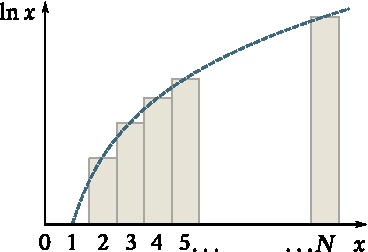
\includegraphics[scale=1]{figures/appendix/fig_A_1.pdf}
		\caption[]{}
		\label{fig:A_1}
	\end{center}
\end{figure}

\noindent
The sum we have written equals the sum of the areas of the columns depicted in \fig{A_1}. At great values of N, the sum of the areas of
these columns differs very slightly from the area confined by the dash curve, which is a graph of the function $\ln{x}$. Hence,
\begin{equation*}
    \ln{N!} \approx \int_1^N \ln{x}\,\deriv{x} = [x\ln{x} - x]_1^N = N\ln{N} - N + 1.
\end{equation*}

\noindent
With great values of $N$, we may disregard unity, and we arrive at the formula
\begin{equation}\label{eq:A_7}
    \ln{N!} \approx N \ln{N} - N
\end{equation}

\noindent
which is called the \textbf{Stirling formula}.

We must note that, strictly speaking, the Stirling formula has another addend equal to $\ln(2\pi N)/2$. With great values of $N$, however, this addend may be disregarded in comparison with the other two addends.
